
\pdfminorversion=4 % for acroread
%\documentclass[aspectratio=169,t,xcolor={usenames,dvipsnames}]{beamer}
\documentclass[aspectratio=169,t,handout,xcolor={usenames,dvipsnames}]{beamer}
\usepackage{../beamerstyle}
\usepackage{dsfont}
\usepackage{bm}
\usepackage[english]{babel}
\usepackage[utf8]{inputenc}
\usepackage{graphicx}
\usepackage{algorithm}
\usepackage[ruled,vlined,algo2e,linesnumbered]{algorithm2e}
%\usepackage[boxed,vlined]{algorithm2e}
\usepackage{hyperref}
\usepackage{booktabs}
\usepackage{mathtools}

\usepackage{amsmath,amssymb}
\usepackage{listings}
\lstset{frame=lines,framesep=3pt,numbers=left,numberblanklines=false,basicstyle=\ttfamily\small}

\usepackage{subfig}
\usepackage{multicol}
%\usepackage{appendixnumberbeamer}
%
\usepackage{tcolorbox}

\usepackage{pgfplots}
\usepackage{tikz}
\usetikzlibrary{trees} 
\usetikzlibrary{shapes.geometric}
\usetikzlibrary{positioning,shapes,shadows,arrows,calc,mindmap}
\usetikzlibrary{positioning,fadings,through}
\usetikzlibrary{decorations.pathreplacing}
\usetikzlibrary{intersections}
\usetikzlibrary{positioning,fit,calc,shadows,backgrounds}
\pgfdeclarelayer{background}
\pgfdeclarelayer{foreground}
\pgfsetlayers{background,main,foreground}
\tikzstyle{activity}=[rectangle, draw=black, rounded corners, text centered, text width=8em]
\tikzstyle{data}=[rectangle, draw=black, text centered, text width=8em]
\tikzstyle{myarrow}=[->, thick, draw=black]

% Define the layers to draw the diagram
\pgfdeclarelayer{background}
\pgfdeclarelayer{foreground}
\pgfsetlayers{background,main,foreground}

%\usepackage{listings}
%\lstset{numbers=left,
%  showstringspaces=false,
%  frame={tb},
%  captionpos=b,
%  lineskip=0pt,
%  basicstyle=\ttfamily,
%%  extendedchars=true,
%  stepnumber=1,
%  numberstyle=\small,
%  xleftmargin=1em,
%  breaklines
%}

 
\definecolor{blue}{RGB}{0, 74, 153}

\usetheme{Boadilla}
%\useinnertheme{rectangles}
\usecolortheme{whale}
\setbeamercolor{alerted text}{fg=blue}
\useoutertheme{infolines}
\setbeamertemplate{navigation symbols}{\vspace{-5pt}} % to lower the logo
\setbeamercolor{date in head/foot}{bg=white} % blue
\setbeamercolor{date in head/foot}{fg=white}
\setbeamercolor{author  in head/foot}{bg=white} %blue
\setbeamercolor{title in head/foot}{bg=white} % blue
\setbeamercolor{title}{fg=white, bg=blue}
\setbeamercolor{block title}{fg=white,bg=blue}
\setbeamercolor{block body}{bg=blue!10}
\setbeamercolor{frametitle}{fg=white, bg=blue}
\setbeamercovered{invisible}

\makeatletter
\setbeamertemplate{footline}
{
  \leavevmode%
  \hbox{%
  \begin{beamercolorbox}[wd=.333333\paperwidth,ht=2.25ex,dp=1ex,center]{author in head/foot}%
%    \usebeamerfont{author in head/foot}\insertshortauthor
  \end{beamercolorbox}%
  \begin{beamercolorbox}[wd=.333333\paperwidth,ht=2.25ex,dp=1ex,center]{title in head/foot}%
    \usebeamerfont{title in head/foot}\insertshorttitle
  \end{beamercolorbox}%
  \begin{beamercolorbox}[wd=.333333\paperwidth,ht=2.25ex,dp=1ex,right]{date in head/foot}%
    \usebeamerfont{date in head/foot}\insertshortdate{}\hspace*{2em}
%    \insertframenumber\hspace*{2ex} 
  \end{beamercolorbox}}%
  \vskip0pt%
}
\makeatother

%\pgfdeclareimage[height=1.2cm]{automl}{images/logos/automl.png}
%\pgfdeclareimage[height=1.2cm]{freiburg}{images/logos/freiburg}

%\logo{\pgfuseimage{freiburg}}

\renewcommand{\comment}[1]{
	\noindent
	%\vspace{0.25cm}
	{\color{red}{\textbf{TODO:} #1}}
	%\vspace{0.25cm}
}
\newcommand{\notefh}[1]{\textcolor{red}{\textbf{FH:} #1}}
\renewcommand{\comment}[1]{}
\newcommand{\hide}[1]{}
\newcommand{\cemph}[2]{\emph{\textcolor{#1}{#2}}}

\newcommand{\lit}[1]{{\footnotesize\color{black!60}[#1]}}

\newcommand{\litw}[1]{{\footnotesize\color{blue!20}[#1]}}


\newcommand{\myframe}[2]{\begin{frame}[c]{#1}#2\end{frame}}
\newcommand{\myframetop}[2]{\begin{frame}{#1}#2\end{frame}}
\newcommand{\myit}[1]{\begin{itemize}#1\end{itemize}}
\newcommand{\myblock}[2]{\begin{block}{#1}#2\end{block}}


\newcommand{\votepurple}[1]{\textcolor{Purple}{$\bigstar$}}
\newcommand{\voteyellow}[1]{\textcolor{Goldenrod}{$\bigstar$}}
\newcommand{\voteblue}[1]{\textcolor{RoyalBlue}{$\bigstar$}}
\newcommand{\votepink}[1]{\textcolor{Pink}{$\bigstar$}}

\newcommand{\diff}{\mathop{}\!\mathrm{d}}
\newcommand{\refstyle}[1]{{\small{\textcolor{gray}{#1}}}}
\newcommand{\hands}[0]{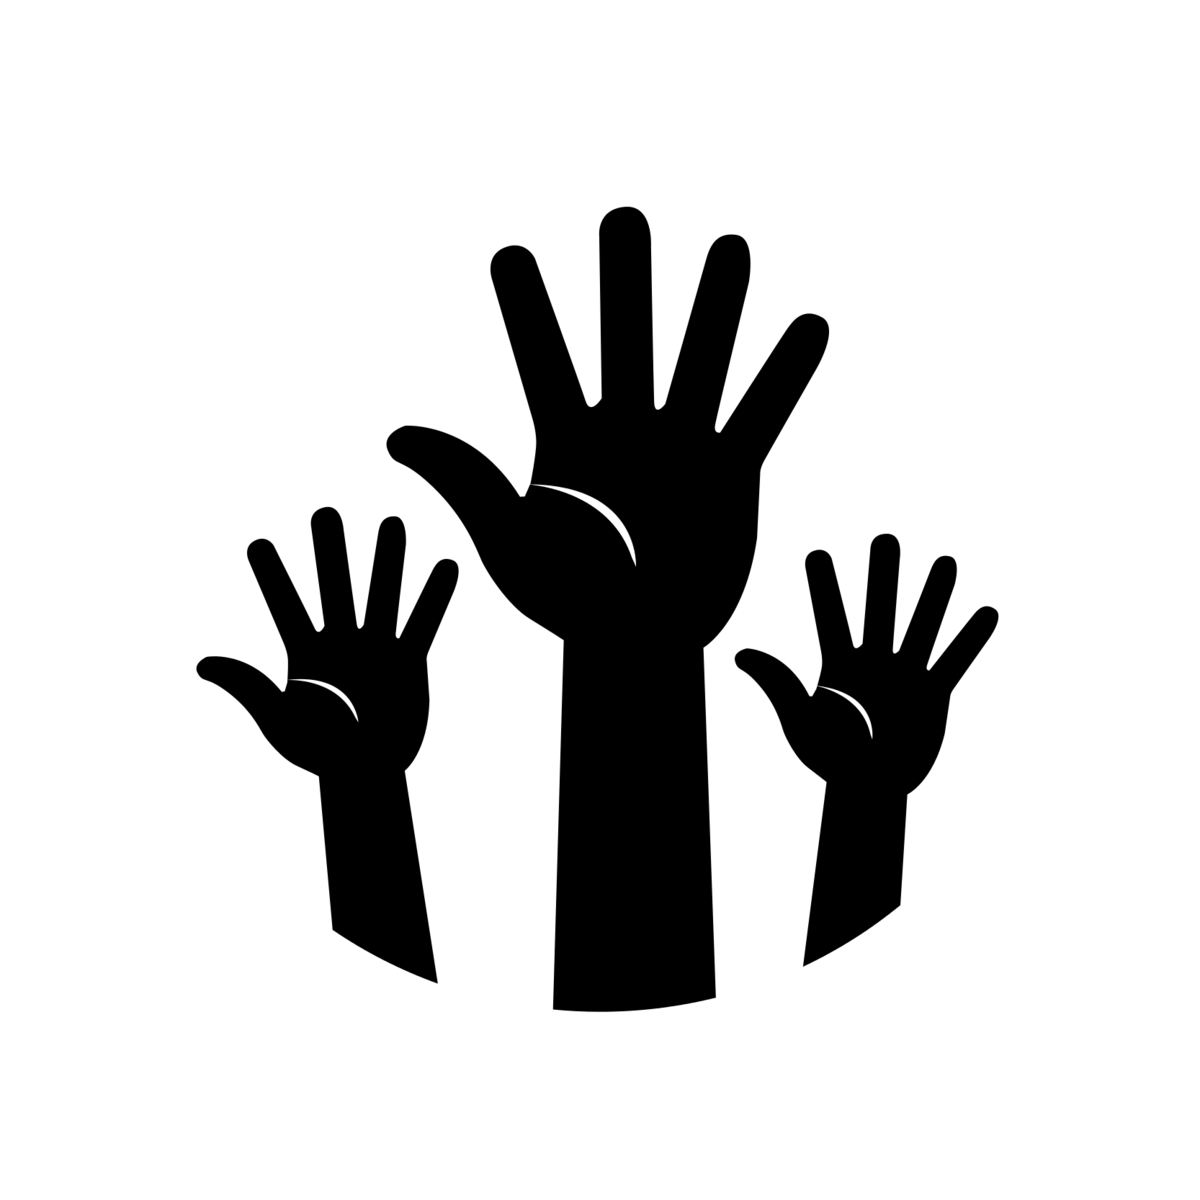
\includegraphics[height=1.5em]{images/hands}}
\newcommand{\transpose}[0]{{\textrm{\tiny{\sf{T}}}}}
\newcommand{\norm}{{\mathcal{N}}}
\newcommand{\cutoff}[0]{\kappa}
\newcommand{\instD}[0]{\dataset}
\newcommand{\insts}[0]{\mathcal{I}}
\newcommand{\inst}[0]{i}
\newcommand{\instI}[1]{i^{(#1)}}

% Iteration specific instance of variable/function/anything
% Introduced in the BO section, but moved up here to make it available within other macros
\newcommand{\iter}[2][\bocount]{{#2}^{(#1)}}

%--------HPO parameter macros-----------

% Parameter Configuration Space
\newcommand{\pcs}[0]{\pmb{\Lambda}}

% ???
\newcommand{\bx}[0]{\conf}

% Parameter Configuration
\newcommand{\conf}[0]{\pmb{\lambda}}

% Final Configuration
\newcommand{\finconf}[0]{\pmb{\hat{\lambda}}}

% Configuration corresponding to a given iteration -- better use \iter!
\newcommand{\confI}[1]{{\conf}^{(#1)}}

% Default Configuration
\newcommand{\defconf}[0]{{\conf}_{\text{def}}}

% Incumbent Configuration
\newcommand{\incumbent}[1][\bocount]{\iter[#1]{\finconf}}

% Optimal Configuration
\newcommand{\optconf}[0]{{\conf}^*}

% Configuration Space
\newcommand{\confs}[0]{\pcs}

%----------------------------------------

%\newcommand{\vlambda}[0]{\bm{\lambda}}
%\newcommand{\vLambda}[0]{\bm{\Lambda}}
\newcommand{\dataset}[0]{\mathcal{D}}
\newcommand{\datasets}[0]{\mathbf{D}}
\newcommand{\loss}[0]{L}
\newcommand{\risk}{\mathcal{R}}
\newcommand{\riske}{\mathcal{R}_{\text{emp}}}
\newcommand{\cost}[0]{c}
\newcommand{\costI}[1]{c^{(#1)}}

% Gaussian Process
\newcommand{\gp}{\mathcal{G}}
% Family of Objective Functions
\newcommand{\objF}{F}

%---------------BO Macros------------------

% BO loop counter
\newcommand{\bocount}{t}
% BO loop counter max, the counter runs from 1 to this value
\newcommand{\bobudget}{T}
% BO loop observation
\newcommand{\obs}[1][\conf]{\cost({#1})}
% BO loop observation space
\newcommand{\obsspace}{\mathcal{Y}}
% BO loop next observation
\newcommand{\bonextobs}{\obs[\iter{\conf}]}
% Acquisition Function, no args
\newcommand{\acq}{u}
% Standard Normal PDF
\newcommand{\pdf}{\phi}
% Standard Normal CDF
\newcommand{\cdf}{\Phi}
% Mean
\newcommand{\mean}{\mu}
% Standard Deviation
\newcommand{\stddev}{\sigma}
% Variance
\newcommand{\variance}{\sigma^2}
% Noise
\newcommand{\noise}{\nu}
% BO loop next selected sample
\newcommand{\bonextsample}{\confI{\bocount}}

% Single hyperparameter
\newcommand{\hyperparam}{\lambda}

% Single hyperparameter within a hyperparameter configuration
\newcommand{\hyperparami}[1][i]{{\hyperparam}_#1}

% Full definition of final configuration
\newcommand{\finconffull}{\incumbent[\bobudget]}

% Dataset
\newcommand{\datasetHPO}{{\dataset}_{HPO}}

% Dataset definition
\newcommand{\datasetHPOdef}{{\langle \bonextsample,\,\bonextobs \rangle}_{\bocount=1}^{\bobudget}}

% Double Display Fraction, forces large displays for everything in numerator and denominator
\newcommand\ddfrac[2]{\frac{\displaystyle #1}{\displaystyle #2}}

% Conditional Probability "Given That" Relation, source:https://tex.stackexchange.com/a/141685/205886
\newcommand\given[1][]{\:#1\vert\:}

% Expectation as a math operator
\DeclareMathOperator*{\E}{\mathbb{E}}

% Citation 
\newcommand{\source}[1]{
    \begin{flushright}
    	Source: \lit{#1}
    \end{flushright}
}
%-------------------------------------------

%Real numbers set
\newcommand{\realnum}{\mathbb{R}}
%Configuration space - do not use
%\newcommand{\configspace}{\Theta}
%Instances - do not use
%\newcommand{\instances}{\mathcal{I}}
%Expected value
\newcommand{\expectation}{\mathbb{E}}
%Kernel
\newcommand{\kernel}{\kappa}
%Constraint function
\newcommand{\constraintf}{c}
%Normal distribution
\newcommand{\normaldist}{\mathcal{N}}

% \renewcommand{\vec}[1]{\mathbf{#1}}
\newcommand{\hist}[0]{\dataset_{\text{Hist}}}
\newcommand{\param}[0]{p}
\newcommand{\algo}[0]{\mathcal{A}}
\newcommand{\algos}[0]{\mathbf{A}}
%\newcommand{\nn}[0]{N}
\newcommand{\feats}[0]{\mathcal{X}_{\text{meta}}}
\newcommand{\feat}[0]{\x_{\text{meta}}}
%\newcommand{\cluster}[0]{\vec{h}}
%\newcommand{\clusters}[0]{\vec{H}}
\newcommand{\perf}[0]{\mathbb{R}}
%\newcommand{\surro}[0]{\mathcal{S}}
\newcommand{\surro}[0]{\hat{\cost}}
\newcommand{\func}[0]{f}
\newcommand{\epm}[0]{\surro}
\newcommand{\portfolio}[0]{\mathbf{P}}
\newcommand{\schedule}[0]{\mathcal{S}}

% Machine Learning
\newcommand{\mdata}[0]{\dataset_{\text{meta}}}
\newcommand{\datasettrain}[0]{\dataset_{\text{train}}}
\newcommand{\datasetval}[0]{\dataset_{\text{val}}}
\newcommand{\datasettest}[0]{\dataset_{\text{test}}}
\newcommand{\x}[0]{\mathbf{x}}
\newcommand{\y}[0]{y}
\newcommand{\xI}[1]{\mathbf{x}^{(#1)}}
\newcommand{\yI}[1]{y^{(#1)}}
\newcommand{\fx}{f(\mathbf{x})}  % f(x), continuous prediction function
\newcommand{\Hspace}{\mathcal{H}} % hypothesis space where f is from
\newcommand{\fh}{\hat{f}}       % f hat, estimated prediction function

% Deep Learning
\newcommand{\weights}[0]{\theta}
\newcommand{\metaweights}[0]{\phi}


% reinforcement learning
\newcommand{\policies}[0]{\mathbf{\Pi}}
\newcommand{\policy}[0]{\pi}
\newcommand{\actionRL}[0]{a}
\newcommand{\stateRL}[0]{s}
\newcommand{\statesRL}[0]{\mathcal{S}}
\newcommand{\rewardRL}[0]{r}
\newcommand{\rewardfuncRL}[0]{\mathcal{R}}

\RestyleAlgo{algoruled}
\DontPrintSemicolon
\LinesNumbered
\SetAlgoVlined
\SetFuncSty{textsc}

\SetKwInOut{Input}{Input}
\SetKwInOut{Output}{Output}
\SetKw{Return}{return}

%\newcommand{\changed}[1]{{\color{red}#1}}

%\newcommand{\citeN}[1]{\citeauthor{#1}~(\citeyear{#1})}

\renewcommand{\vec}[1]{\mathbf{#1}}
\DeclareMathOperator*{\argmin}{arg\,min}
\DeclareMathOperator*{\argmax}{arg\,max}

%\newcommand{\aqme}{\textit{AQME}}
%\newcommand{\aslib}{\textit{ASlib}}
%\newcommand{\llama}{\textit{LLAMA}}
%\newcommand{\satzilla}{\textit{SATzilla}}
%\newcommand{\satzillaY}[1]{\textit{SATzilla'{#1}}}
%\newcommand{\snnap}{\textit{SNNAP}}
%\newcommand{\claspfolioTwo}{\textit{claspfolio~2}}
%\newcommand{\flexfolio}{\textit{FlexFolio}}
%\newcommand{\claspfolioOne}{\textit{claspfolio~1}}
%\newcommand{\isac}{\textit{ISAC}}
%\newcommand{\eisac}{\textit{EISAC}}
%\newcommand{\sss}{\textit{3S}}
%\newcommand{\sunny}{\textit{Sunny}}
%\newcommand{\ssspar}{\textit{3Spar}}
%\newcommand{\cshc}{\textit{CSHC}}
%\newcommand{\cshcpar}{\textit{CSHCpar}}
%\newcommand{\measp}{\textit{ME-ASP}}
%\newcommand{\aspeed}{\textit{aspeed}}
%\newcommand{\autofolio}{\textit{AutoFolio}}
%\newcommand{\cedalion}{\textit{Cedalion}}
\newcommand{\fanova}{\textit{fANOVA}}
\newcommand{\sbs}{\textit{SB}}
\newcommand{\oracle}{\textit{VBS}}

% like approaches
\newcommand{\claspfoliolike}[1]{\texttt{claspfolio-#1-like}}
\newcommand{\satzillalike}[1]{\texttt{SATzilla'#1-like}}
\newcommand{\isaclike}{\texttt{ISAC-like}}
\newcommand{\ssslike}{\texttt{3S-like}}
\newcommand{\measplike}{\texttt{ME-ASP-like}}

\newcommand{\irace}{\textit{I/F-race}}
\newcommand{\gga}{\textit{GGA}}
\newcommand{\smac}{\textit{SMAC}}
\newcommand{\paramils}{\textit{ParamILS}}
\newcommand{\spearmint}{\textit{Spearmint}}
\newcommand{\tpe}{\textit{TPE}}


\usepackage{pifont}
\newcommand{\itarrow}{\mbox{\Pisymbol{pzd}{229}}}
\newcommand{\ithook}{\mbox{\Pisymbol{pzd}{52}}}
\newcommand{\itcross}{\mbox{\Pisymbol{pzd}{56}}}
\newcommand{\ithand}{\mbox{\raisebox{-1pt}{\Pisymbol{pzd}{43}}}}

%\DeclareMathOperator*{\argmax}{arg\,max}

\newcommand{\ie}{{\it{}i.e.\/}}
\newcommand{\eg}{{\it{}e.g.\/}}
\newcommand{\cf}{{\it{}cf.\/}}
\newcommand{\wrt}{\mbox{w.r.t.}}
\newcommand{\vs}{{\it{}vs\/}}
\newcommand{\vsp}{{\it{}vs\/}}
\newcommand{\etc}{{\copyedit{etc.}}}
\newcommand{\etal}{{\it{}et al.\/}}

\newcommand{\pscProc}{{\bf procedure}}
\newcommand{\pscBegin}{{\bf begin}}
\newcommand{\pscEnd}{{\bf end}}
\newcommand{\pscEndIf}{{\bf endif}}
\newcommand{\pscFor}{{\bf for}}
\newcommand{\pscEach}{{\bf each}}
\newcommand{\pscThen}{{\bf then}}
\newcommand{\pscElse}{{\bf else}}
\newcommand{\pscWhile}{{\bf while}}
\newcommand{\pscIf}{{\bf if}}
\newcommand{\pscRepeat}{{\bf repeat}}
\newcommand{\pscUntil}{{\bf until}}
\newcommand{\pscWithProb}{{\bf with probability}}
\newcommand{\pscOtherwise}{{\bf otherwise}}
\newcommand{\pscDo}{{\bf do}}
\newcommand{\pscTo}{{\bf to}}
\newcommand{\pscOr}{{\bf or}}
\newcommand{\pscAnd}{{\bf and}}
\newcommand{\pscNot}{{\bf not}}
\newcommand{\pscFalse}{{\bf false}}
\newcommand{\pscEachElOf}{{\bf each element of}}
\newcommand{\pscReturn}{{\bf return}}

%\newcommand{\param}[1]{{\sl{}#1}}
\newcommand{\var}[1]{{\it{}#1}}
\newcommand{\cond}[1]{{\sf{}#1}}
%\newcommand{\state}[1]{{\sf{}#1}}
%\newcommand{\func}[1]{{\sl{}#1}}
\newcommand{\set}[1]{{\Bbb #1}}
%\newcommand{\inst}[1]{{\tt{}#1}}
\newcommand{\myurl}[1]{{\small\sf #1}}

\newcommand{\Nats}{{\Bbb N}}
\newcommand{\Reals}{{\Bbb R}}
\newcommand{\extset}[2]{\{#1 \; | \; #2\}}

\newcommand{\vbar}{$\,\;|$\hspace*{-1em}\raisebox{-0.3mm}{$\,\;\;|$}}
\newcommand{\vendbar}{\raisebox{+0.4mm}{$\,\;|$}}
\newcommand{\vend}{$\,\:\lfloor$}


\newcommand{\goleft}[2][.7]{\parbox[t]{#1\linewidth}{\strut\raggedright #2\strut}}
\newcommand{\rightimage}[2][.3]{\mbox{}\hfill\raisebox{1em-\height}[0pt][0pt]{\includegraphics[width=#1\linewidth]{#2}}\vspace*{-\baselineskip}}





\usepackage{multirow}


\title[AutoML: Risks]{AutoML: Evaluation} % week title
\subtitle{Benchmarking and Comparing Learners} % video title
\author[Lars Kotthoff]{\underline{Bernd Bischl} \and Frank Hutter \and \underline{Lars Kotthoff}\newline \and Marius Lindauer \and Joaquin Vanschoren}
\institute{}
\date{}

\newcommand\reffootnote[1]{%
    \begingroup
    \renewcommand\thefootnote{}\footnote{
        \tiny #1
    \vspace*{1em}}%
    \addtocounter{footnote}{-1}%
    \endgroup
}

% \AtBeginSection[] % Do nothing for \section*
% {
%   \begin{frame}{Outline}
%     \bigskip
%     \vfill
%     \tableofcontents[currentsection]
%   \end{frame}
% }

\begin{document}
	
	\maketitle

    \begin{frame}[c]{Benchmark Experiments}

    \begin{itemize}
    \item different learning algorithms applied to one or more data sets to compare and rank their performances
    \item synchronized train and test sets, i.e.\ the same resampling method
        with the same train-test splits should be used to determine performance
    \newline
    \textbf{Example}: Benchmark results (per CV-fold) of CART and random forest using 2-fold CV with MSE as performance measure:
    \medskip

    \begin{center}
        \scriptsize
        \begin{tabular}{cccc}
        \toprule
        data set & k-th fold & MSE (rpart) & MSE (randomForest)\\
        \midrule
        BostonHousing & 1 & 29.4 & 17.13\\
        BostonHousing & 2 & 20.5 & 8.90\\
        mtcars & 1 & 35.0 & 7.53\\
        mtcars & 2 & 38.9 & 6.73\\
        \bottomrule
        \end{tabular}
    \end{center}
    \end{itemize}

    \end{frame}

    \begin{frame}[c,allowframebreaks]{Hypothesis Testing in Benchmarking}
    We want to know if the difference in performance between models (or algorithms) is significant or only by chance.

    \textbf{Null Hypothesis Statistical Testing (NHST)} in Benchmarking:

    \begin{itemize}
    \item formulate null hypothesis $H_0$ (e.g.\ the expected generalization
        error of two algorithms is equivalent) and alternative hypothesis $H_1$
    \item use hypothesis test to reject $H_0$ (not rejecting $H_0$ does not mean that we accept it)
    \item rejecting $H_0$ gives some confidence that the observed results may
        not be random
    \end{itemize}

    Typical example in machine learning:

    \begin{itemize}
    \item $H_0$: on average, model 1 does not perform better than model 2
    \item $H_1$: on average, model 1 outperforms the model 2
    \item Aim: Reject $H_0$ with confidence level of $1-\alpha$ (common values
        for $\alpha$ include 0.05 and 0.01)
    \end{itemize}

    \framebreak

    Selection of an appropriate hypothesis test is at least based on the type of
    problem, i.e.\ if the aim is to compare
    \begin{itemize}
    \item 2 models / algorithms on a single domain (i.e.\ on a single data set)
    \item 2 algorithms across different domains (i.e.\ on multiple data sets)
    \item multiple algorithms across different domains / data sets
    \end{itemize}

    \begin{center}
    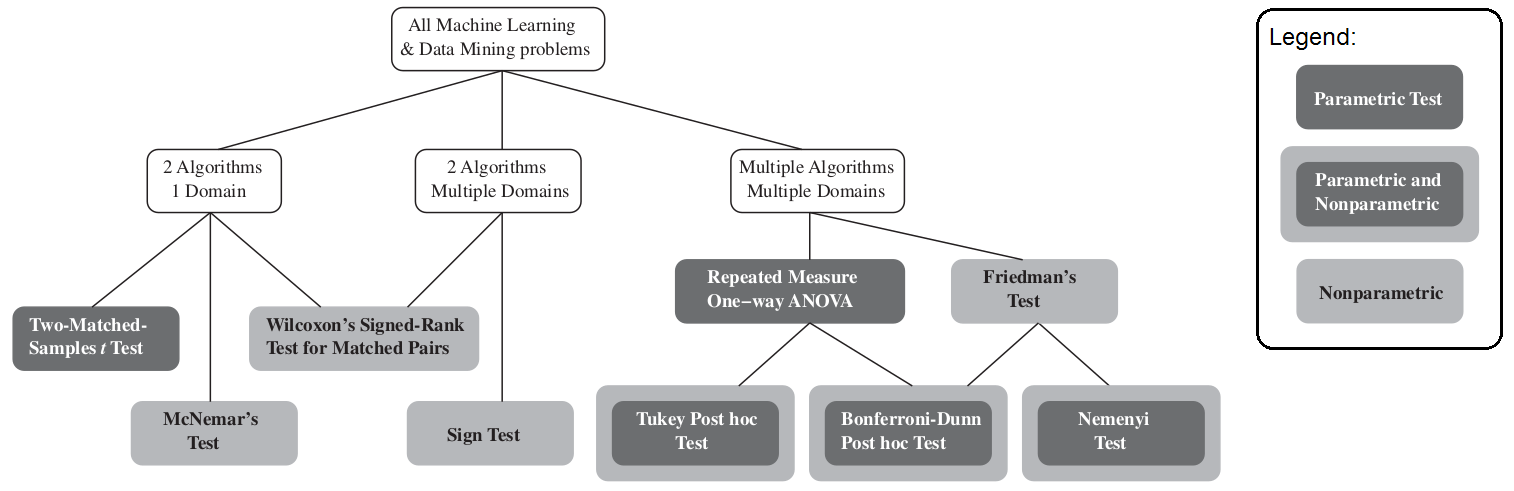
\includegraphics[height=.5\textheight]{tests_overview.png}
    \end{center}

    \end{frame}

    \begin{frame}[c,allowframebreaks]{McNemar Test}
    \begin{itemize}
    \item non-parametric test used on paired nominal data, does not make any distributional assumptions
    \item pairs are e.g.\ performance numbers of different models on the same data
    \item can be applied to compare the performance of two \textbf{models}
        when the considered performance measure is based on an outer loss with a
        nominal or binary output, e.g.\ accuracy is based on a binary outer loss
    \item both models trained on training set and evaluated on test set;
        \textbf{contingency table} based on test set that compares the two models calculated
    \end{itemize}

    \medskip
    \begin{minipage}{0.25\textwidth}
    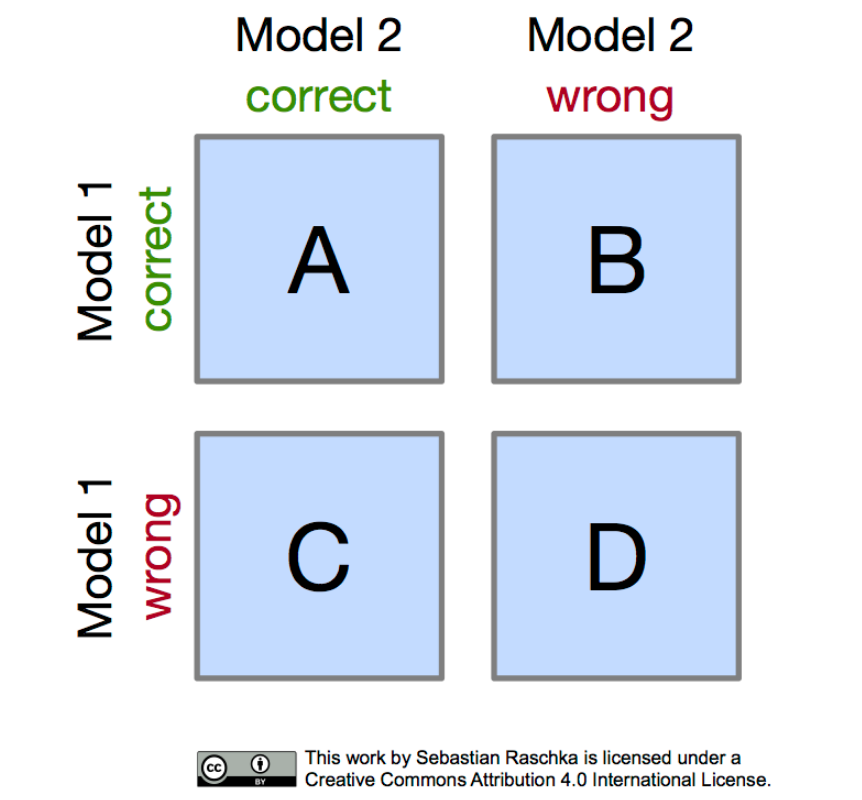
\includegraphics[width=\textwidth]{mcnemar_1.png}
    \end{minipage}
    \begin{minipage}{0.74\textwidth}
    \begin{itemize}
    \item A: $\#$obs.\ misclassified by both.
    \item B: $\#$obs.\ misclassified by model 1 but not by model 2
    \item C: $\#$obs.\ misclassified by model 2 but not by model 1
    \item D: $\#$obs.\ correctly classified by both
    \end{itemize}
    \end{minipage}

    \framebreak

    \begin{minipage}[c]{0.625\linewidth}
    Accuracy of each model can be computed as follows:
    \begin{itemize}
      \item Model 1: (A+B)/(A+B+C+D)
      \item Model 2: (A+C)/(A+B+C+D)
    \end{itemize}

    Even if the models have the \textbf{same} accuracies (indicating equal performance), cells B and C may be different because the models may misclassify different instances.
    \end{minipage}
    \begin{minipage}[c]{0.2\linewidth}
        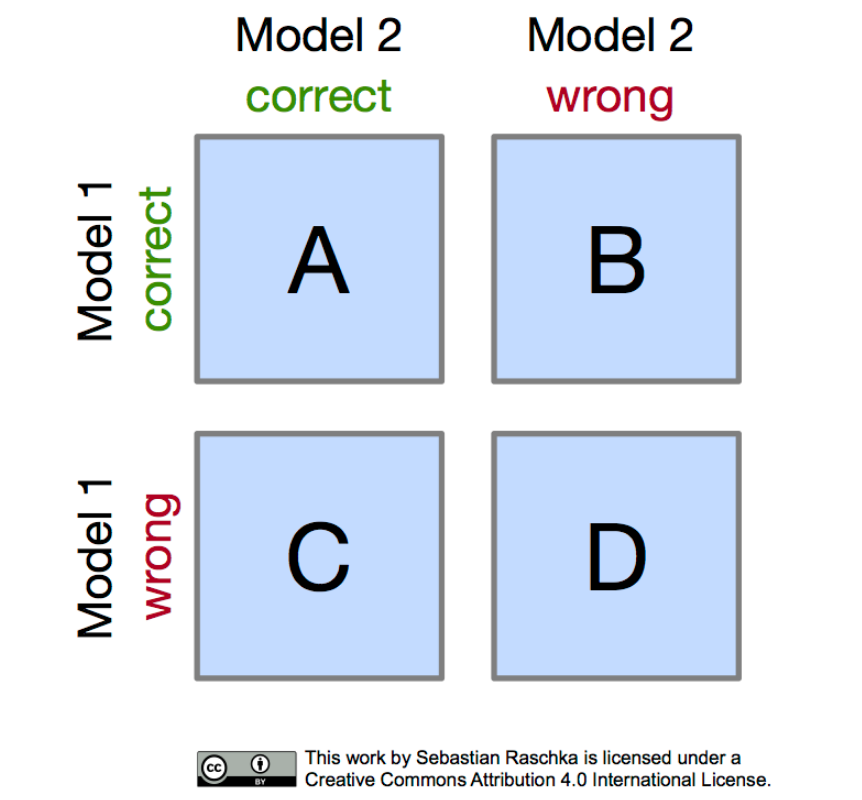
\includegraphics[width=\textwidth]{mcnemar_1.png}
    \end{minipage}

    \medskip

    McNemar tests the following hypothesis:
    \begin{itemize}
    \item $H_0:$ both models have the same performance (we expect B = C)
    \item $H_1:$ performances of the two models are not equal
    \end{itemize}

    The test statistic is computed as
    $$\chi^2_{Mc} =  \tfrac{(|B-C| - 1)^2}{B + C} \sim \chi^2_{1}.$$

    \textbf{Note}: The McNemar test should only be used if $B + C > 20$.

    \framebreak

    \textbf{Example}:

    \begin{center}
      \begin{tabular}{cc|cc}
          & & \multicolumn{2}{c}{Random Forest} \\
          & & $0$ & $1$ \\
          \hline
          \multirow{2}{*}{Tree} & $0$ & 30 & 5 \\
          & $1$ & 17 & 42 \\
      \end{tabular}
    \end{center}

    Calculating the test statistic:

    $$\chi^2_{Mc} =  \frac{(|5-17| - 1)^2}{5 + 17} = 5.5 > 3.841 = \chi^2_{1,0.95}$$

    We can reject $H_0$ at a significance level of 0.05, i.e.\ we reject the hypothesis that the tree and the random forest have the same performance.

    Significance level must be chosen before applying the test (avoid p-value
    hacking).
    \end{frame}


    \begin{frame}[c,allowframebreaks]{Two-Matched-Samples t-Test}

        \begin{itemize}
            \item two-matched-samples t-test (i.e.\ a paired t-test) is the simplest
                hypothesis test to compare two \textbf{models} on a single
                test set based on arbitrary performance measures
            \item parametric test and distributional assumptions must be made
                (which are often problematic):
                \begin{description}
                \item[(pseudo-)normality] usually met when sample size $>$ 30
                \item[i.i.d.\ samples] usually met if loss of individual observations from single test set considered
                \item[equal variances of populations] can be investigated through plots
                \end{description}
        \end{itemize}

    \framebreak

    Compare two different models $\fh_1$ and $\fh_2$ w.r.t.\ performance measure calculated on test set of size $n_{\text{test}}$:

    \begin{itemize}
    \item $H_0$: $GE(\fh_{1}) = GE(\fh_{2})$ vs.\ $H_1$: $GE(\fh_{1}) \neq GE(\fh_{2})$
    \item test statistic $T = \sqrt{n_{\text{test}}}
        \frac{\bar{d}}{\sigma_{d}}$ where
    \begin{itemize}
    \item mean performance difference of both models is
        $\bar{d} = \hat{GE}_{\datasettest}(\fh_{1}) - \hat{GE}_{\datasettest}(\fh_{2})$
    \item standard deviation of this mean difference is
    $$\sigma_{d} = \sqrt{\frac{1}{n_{\text{test}} - 1}\sum_{i=1}^{n_{\text{test}}} \left(d_i - \bar{d} \right)^2},$$
    where $d_i = L(\yI{i}, \fh_1 (\xI{i})) - L(\yI{i}, \fh_2 (\xI{i}))$ and $\bar{d} = \sum\limits_{i=1}^{n_{\text{test}}} d_i$
    \end{itemize}
    \end{itemize}

    \textbf{Note}: $d_i$ is the difference of the outer loss of individual observations from the test set between the two models to be compared.

    \begin{itemize}
    \item could also use a \textbf{$k$-fold CV paired t-test} to compare two \textbf{algorithms} (instead of two models) on single data set
    \item instead of comparing outer loss of individual observations, compare
        generalization errors per CV fold (i.e.\ $k$ generalization errors for
        $k$ CV folds)
    \item performance differences are not independent across CV folds due to
        overlapping training sets (which violates the assumption of i.i.d.\
        samples)
    \item to partly overcome issue of overlapping training sets across folds, Dietterich\footnote{Dietterich (1998). Approximate statistical tests for comparing supervised classification learning algorithms.} suggests using 5 times 2-fold CV so that at least within each repetition neither training nor test sets overlap
    \end{itemize}
    \end{frame}

    \begin{frame}[c,allowframebreaks]{Friedman Test}
    Compare multiple classifiers on multiple data sets:
    \begin{itemize}
    \item $H_0:$ all algorithms are equivalent in their performance and hence their average ranks should be equal
    \item $H_1:$ the average ranks for at least one algorithm is different
    \end{itemize}

    To evaluate $n$ data sets and $k$ algorithms:

    \begin{itemize}
      \item rank each algorithm on each data set from best-performing algorithm (rank 1) to worst-performing algorithm using any performance measure
      \item $R_{ij}$ is the rank of algorithm $j$ on data set $i$
      \item if there is a $d$-way tie after rank $r$, assign rank of $
          \left[(r+1) + (r+2) + ... + (r+d)\right] /d $ to each tied classifier
    \end{itemize}

    \framebreak

    Can now compute:
    \begin{itemize}
      \item overall mean rank
      $ \bar{R} = \frac{1}{nk} \sum_{i=1}^{n} \sum_{j=1}^{k} R_{ij} $
      \item sum of squares total
      $ SS_{Total} = n \sum_{j=1}^{k} (\bar{R}_{.j} - \bar{R})^2 $ where $\bar{R}_{.j} =  \frac{1}{n} \sum_{i=1}^{n} R_{ij}$
      \item sum of squares error
      $ SS_{Error} = \frac{1}{n(k-1)} \sum_{i=1}^{n} \sum_{j=1}^{k} (R_{ij} - \bar{R})^2$
    \end{itemize}

    Test statistic calculated as:

    $${\chi_F}^2 = \frac{SS_{Total}}{SS_{Error}} \sim \chi_{k-1}^2 \text{ for
    large n ($>$15) and k ($>$5)}$$

    For smaller n and k, the $\chi^2$ approximation is imprecise and a look up of $\chi_F^2$ values that were approximated specifically for the Friedman test is suggested.
    \end{frame}


    \begin{frame}[c,allowframebreaks]{Post-Hoc Tests}
        \begin{itemize}
            \item Friedman test checks if all algorithms are ranked equally
            \item does not allow to identify best-performing algorithm
        \end{itemize}
        $\rightarrow$ post-hoc tests

    \bigskip

    \textbf{Post-hoc Nemenyi test}:
    \begin{itemize}
    \item compares all pairsof algorithms to find best-performing algorithm after $H_0$ of the Friedman-test was rejected
    \item for $n$ data sets and $k$ algorithms, $\frac{n(n-1)}{2}$ comparisons
    \item calculate average rank of algorithm $j$ on all $n$ data sets: $\bar{R}_{.j} =\frac{1}{n} \sum_{i=1}^n R_{ij}$
    \end{itemize}

    For any two algorithms $j_1$ and $j_2$, test statistic computed as:
    $$q = \frac{\bar{R}_{.j_1} - \bar{R}_{.j_2}}{\sqrt{\frac{k(k+1)}{6n}}}$$

    \framebreak

    Critical Difference Plot:
    \begin{itemize}
        \item quick way to see what differences are significant across all
            compared learners
        \item all learners that do not differ by at least the critical
            difference are connected by line
        \item a learner not connected to another learner and of lower rank can
            be considered better according to the chosen significance level
    \end{itemize}

    \begin{center}
        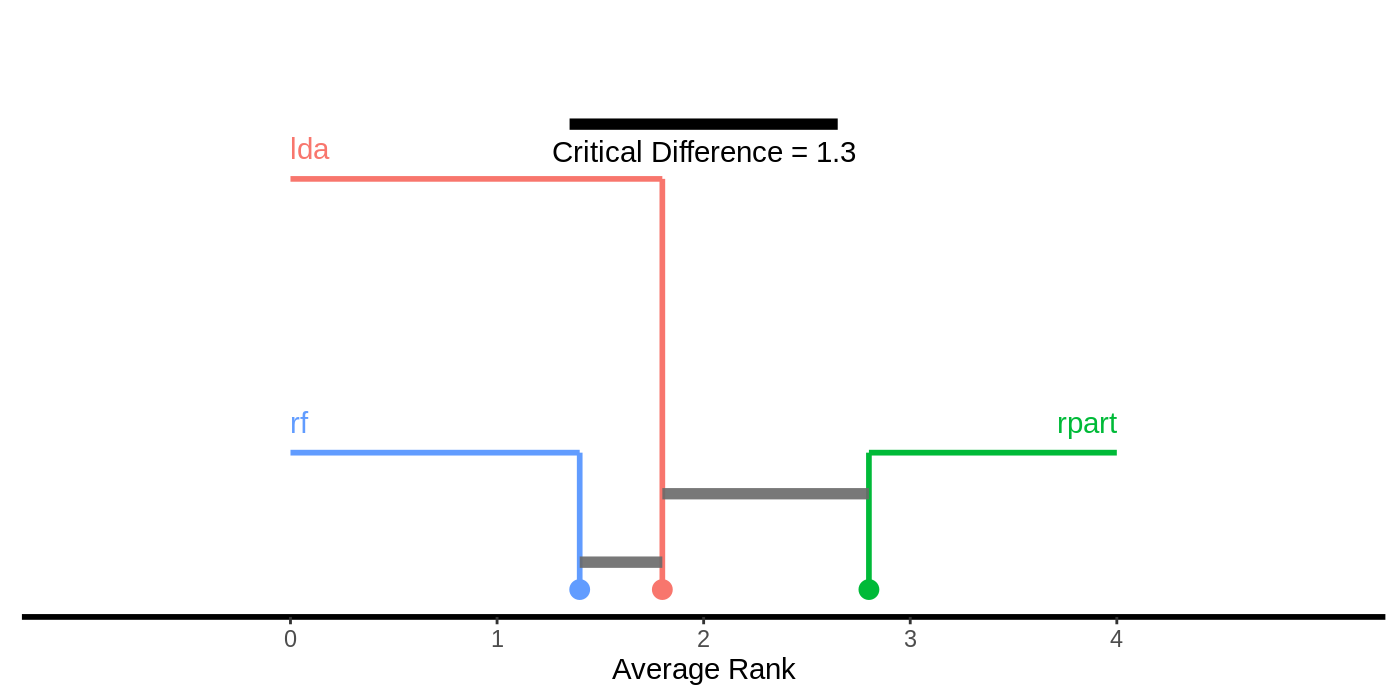
\includegraphics[height=.5\textheight]{crit-diff-nemenyi}
    \end{center}

    \framebreak

    \textbf{Post-hoc Bonferonni-Dunn test}:

    \begin{itemize}
    \item compares all algorithms with baseline (i.e.\ $k-1$ comparisons)
    \item used after Friedman test to find which algorithms differ from the baseline significantly
    \item uses Bonferonni correction to prevent randomly accepting one of the algorithms as significant due to multiple testing
    \end{itemize}
    The test statistic is the same as before:
    $$q = \frac{\bar{R}_{.j_1} - \bar{R}_{.j_2}}{\sqrt{\frac{k(k+1)}{6n}}}.$$

    The performance of $j_1$ and $j_2$ are significantly different when $|q| >
    q_{\alpha}$, where the critical value $q_{\alpha}$ is obtained from a table
    of the studentized range statistic divided by $\sqrt{2}$.

    \framebreak

    \begin{itemize}
        \item learners within the baseline interval (gray line) perform not
            significantly different from the baseline
    \end{itemize}
    \begin{center}
        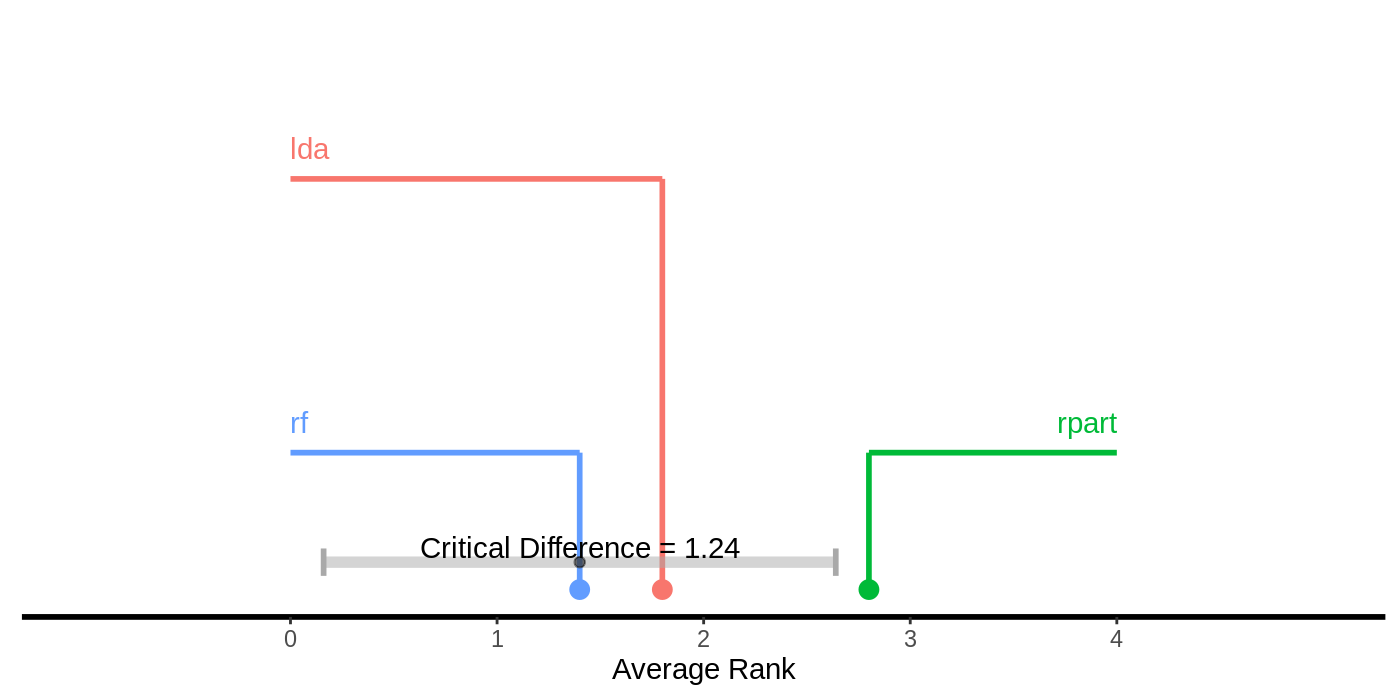
\includegraphics[height=.6\textheight]{crit-diff-bd}
    \end{center}

    \end{frame}

    \begin{frame}[c,allowframebreaks]{Comparing Visually}

    It can be helpful to inspect distributions visually for additional insights,
    e.g.\

    \bigskip
    Boxplots
    \begin{center}
        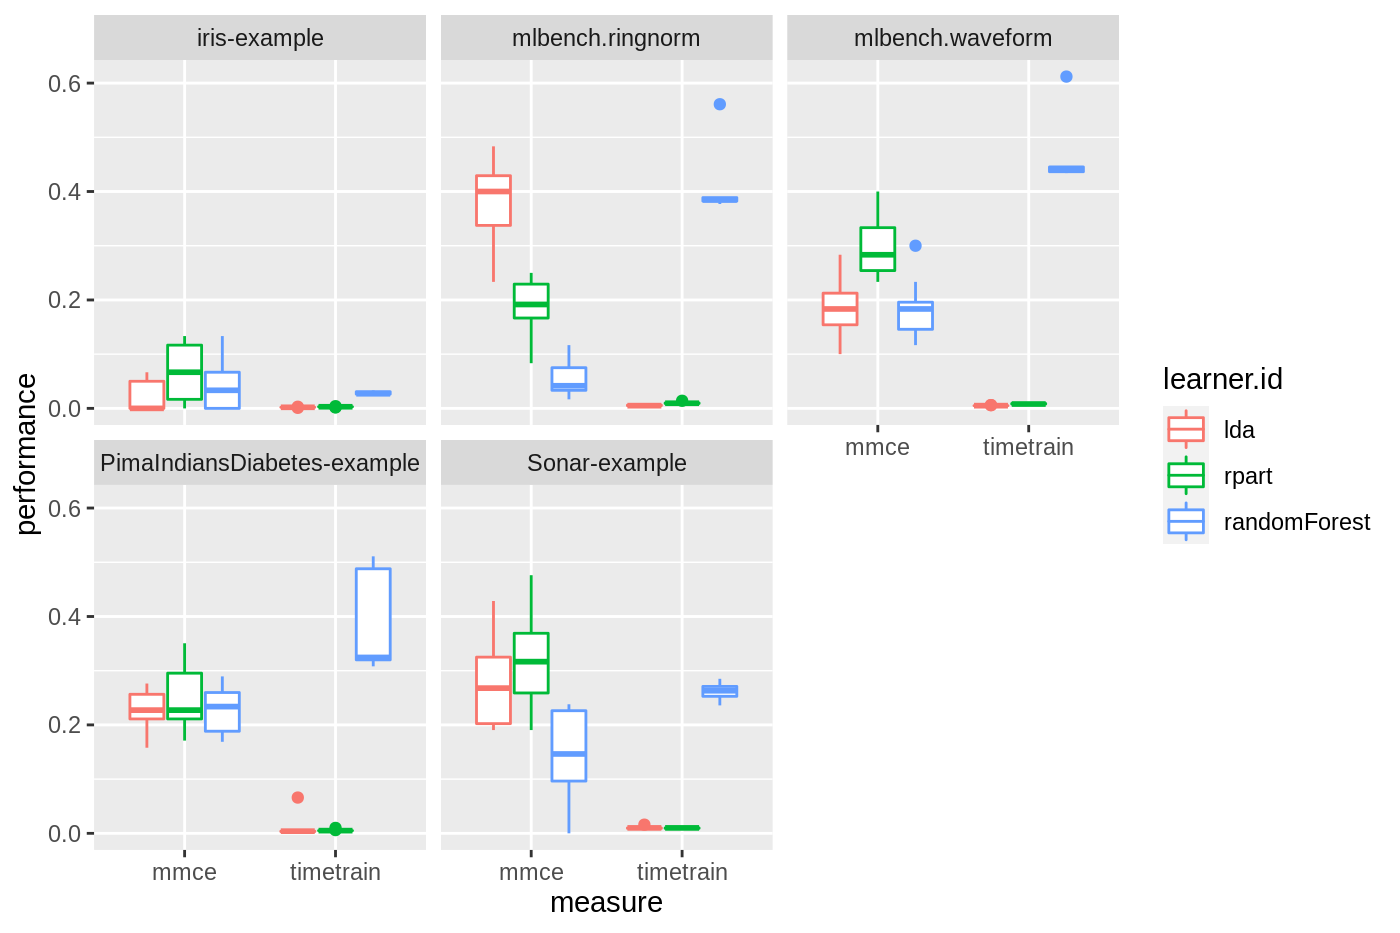
\includegraphics[height=.65\textheight]{multiple-boxplots}
    \end{center}

    \framebreak

    Rank plots
    \begin{center}
        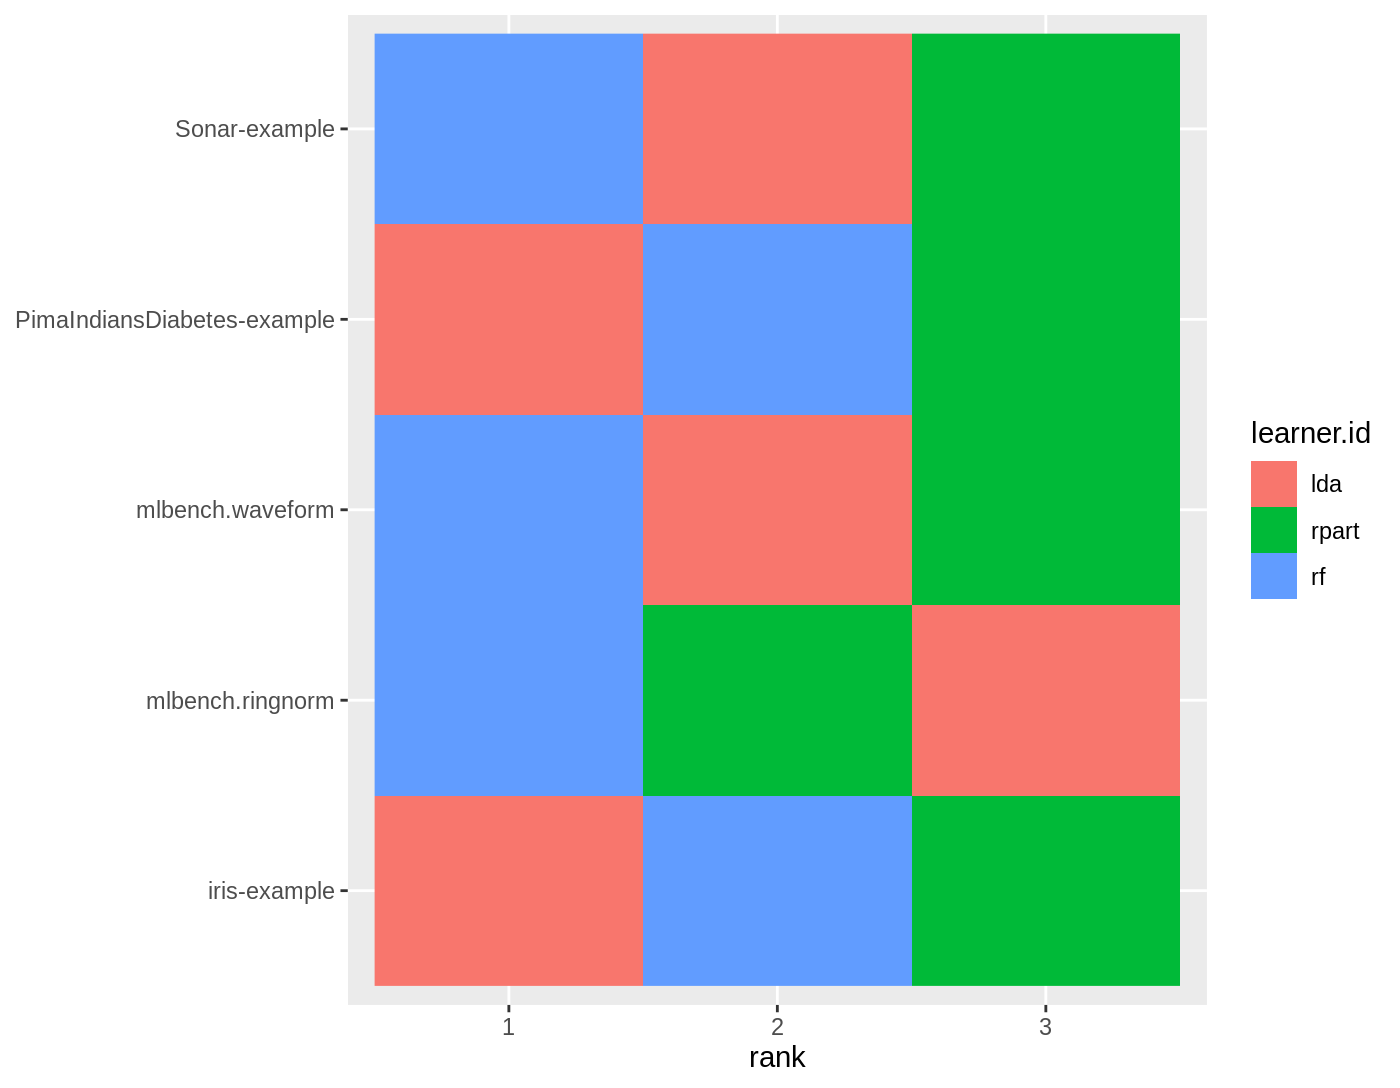
\includegraphics[height=.7\textheight]{multiple-ranks}
    \end{center}

    \end{frame}

\end{document}
